%
% teil3.tex -- Stochastische Differenzialgleichungen
%
% (c) 2023 Lukas Reitemeier, OST Ostschweizer Fachhochschule
%
% !TEX root = ../../buch.tex
% !TEX encoding = UTF-8
%

\section{Stochastische Differenzialgleichungen\label{brown:SDGL}}
\rhead{Stochastische DGL}

Formal kann eine stochastische DGL folgendermaßen notiert werden: 

\begin{equation}
	\label{brown:SDGL:whiteNoise}
	\dot{X}(t) = b(X(t)) + B(X(t))\xi(t) \quad (t>0)
\end{equation}

In diesem Fall ist die Störung durch sogenanntes $ m $ dimensionales weisses Rauschen $ \xi(t) $ modelliert.
$ B $ ist die sogenannte Dispersionsmatrix mit der Dimension $ n $ x $ m $. Sie beschreibt, wie sich die Störung auf die unterschiedlichen inneren Zustände des Systems auswirkt. Dabei beschreibt die Diagonale der Matrix wie stark sich das Rauschen auf jede Dimension auswirkt und die Dreieckberreiche der Matrix beschreiben die Beeinflussung der Dimensionen untereinander.
$ b $ ist der Drift-Vektor und beschreibt die erwartete Veränderung für jeden inneren Zustand / jede Dimension des Systems.
Alles in allem beschreiben $ b $ und $ B $ die Dynamik des Systems. 

\begin{align*}
	b = 
	\begin{pmatrix}
		b_{1} \\
		\vdots \\
		b_{m}\\ 
	\end{pmatrix}
	, \quad
	B = 
	\begin{pmatrix}
		B_{11} & \dots & B_{1m} \\
		& \vdots & \\
		B_{n1} & \dots & B_{nm} 
	\end{pmatrix}
\end{align*}


Für die Modellierung von stochastischem Verhalten, ist der Wiener-Prozess $ W(t) $ ein zentrales Konzept, zumal \textit{White noise} $ \xi(t) $ als die Ableitung vom Wiener-Prozess $ \frac{dW(t)}{dt} $ modelliert werden kann. Somit kann die SDGL aus \ref{brown:SDGL:whiteNoise} folgendermaßen geschrieben werden:

\begin{equation}
	\frac{dX(t)}{dt} = b(X(t)) + B(X(t)) \frac{dW(t)}{dt} \quad (t>0)
\end{equation}

Nun sollte man mit $ dt $  multiplizieren, da die Gleichung sonst impliziert, dass man weisses Rauschen weiter differenzieren kann. Weisses Rauschen $ \frac{dW(t)}{dt} $ ist per Definition nicht sinnvoll weiter differenzierbar. Dies ist den Eigenschaften des Wiener-Prozesses geschuldet. Gemäß der Definition ändert sich die Zufallsvariable in jedem Schritt entsprechend dem Erwartungswert und der Varianz, ohne dabei von vorhergehenden Werten abzuhängen.

Bei SDGLs wird das $ dt $ im Nenner oft mit $ dt $ multipliziert, um die Gleichung in die sogenannte ``Ito-Form'' zu bringen, welche vielfach auch ein erster Schritt im weiteren Umgang ist.

\begin{equation}
	dX(t) = b(X(t)) dt + B(X(t)) dW(t)
\end{equation}


%Man kann dem Wiener Prozess auch fraktale Eigenschaften zusprechen, da man den Ausschnitt des zufällig beeinflussten Prozesses beliebig gross oder klein wählen kann und die keinen Einfluss auf die Eigenschaften des beobachteten Verhalten hat.


\subsection{Simulation mittels der Euler-Maruyama-Methode
	\label{brown:Simulation}}
\rhead{Simulation} %Kurz-Titel der Section

Die brownsche Bewegung kann relativ einfach mittels der Euler-Maruyama-Methode simuliert werden. Diese nummerische Methode wird oft zur Simulation von stochastischen Differentialgleichungen (SDGLs) verwendet und basiert auf der bekannten Euler-Methode zur Lösung von gewöhnlichen Differentialgleichungen. Die Idee ist, die SDGL in diskrete Zeitschritte zu zerlegen und den deterministischen und stochastischen Anteil separat zu behandeln. Die Methode hat zwar gewisse Einschränkungen bezüglich ihrer Genauigkeit und Stabilität, ist aber dennoch mitunter auf Grund ihrer Einfachheit weit verbreitet.

%Gegeben sei eine SDGL der folgenden Form:

%\begin{equation}
%	\mathrm{d}X(t) = a(X(t), t) \mathrm{d}t + b(X(t), t) \mathrm{d}W(t),
%\end{equation}

%wobei $ a(X(t), t) $ den deterministische Anteil darstellt, $ b(X(t), t) $ der stochastische Anteil ist und $ W(t) $ ein Wiener-Prozess ist, welcher das Rauschen repräsentiert. Die Methode beginnt mit einer Anfangsbedingung $X(0) = X_0$.

Um die SDGL mittels der Euler-Maruyama-Methode zu simulieren, geht man wie folgt vor:

\begin{enumerate}
	\item Man wählt eine Schrittweite $ \Delta t > 0 $ und teilt das Zeitintervall $ [0, T] $ in $ N $ gleich große Teilintervalle der Länge $ \Delta t$ : $ t_0 = 0, t_1 = \Delta t, \dots, t_i = i\Delta t, \dots, t_N = T $.
	\item Für jeden Zeitschritt $ i $ von $ 0 $ bis $ N-1 $ werden die Werte der Funktion $ X(t) $ an den diskreten Zeitpunkten $ t_i $ berechnet,
	\begin{equation}
		X(t_{i+1}) = X(t_i) + a(X(t_i), t_i) \Delta t + b(X(t_i), t_i) \sqrt{\Delta t} \cdot Z_i,
	\end{equation}
	wobei $ Z_i $ unabhängige standardnormalverteilte Zufallsvariablen sind.
	\item Diese Berechnungen führt man iterativ für alle Zeitschritte durch.
\end{enumerate}

\begin{equation}
	X_{n+1} = X_n + f(X_n,t_n) \Delta t + g(X_n,t_n) \Delta W_n
\end{equation}

Diese Funktion $ f(X_n,t_n) $ beschreibt den deterministischen Teil der SDGL, im Kontext der brownschen Bewegung kann man es "Drift" nennen, welcher nicht nur von zufälligen Einflüssen bestimmt ist. Man muss jedoch erwähnen, dass er Erwartungswert zu jedem Zeitpunkt dem Startwert entspricht, also der zu erwartende Dritt 0 ist. 


Dies ist auch der Teil, der durch eine harmonische Analyse untersucht werden kann. Das Rauschen (\textit{white noise}), welches hier mit $ g(X_n,t_n) $ beschrieben ist, enthält keine Information und kann somit nicht analysiert werden. $ \Delta W $ beschreibt die Geschwindigkeit, mit welcher der stochastische Prozess ablaufen soll und $ W_n $  beschreibt den Wiener-Prozess oder die brownsche Bewegung als Ganzes.

%Abbildung hier?

In der Abbildung \ref{1Dbrownian} wurde diese Simulations-Methode in einer Dimension angewandt. Man kann vielleicht schon erahnen, dass die zugrundeliegende Mathematik auf Börsenkurse anwendbar sein könnte. Führt man die Simulation für zwei Achsen durch und verbindet die einzelnen Simulationsschritte mit Linien, ergibt sich das Bild einer typischen brownschen Bewegung, wie dies in der Abbildung \ref{2Dbrownian} zu sehen ist.

\begin{figure}
	\centering
	\begin{minipage}{0.45\textwidth}
		\centering
		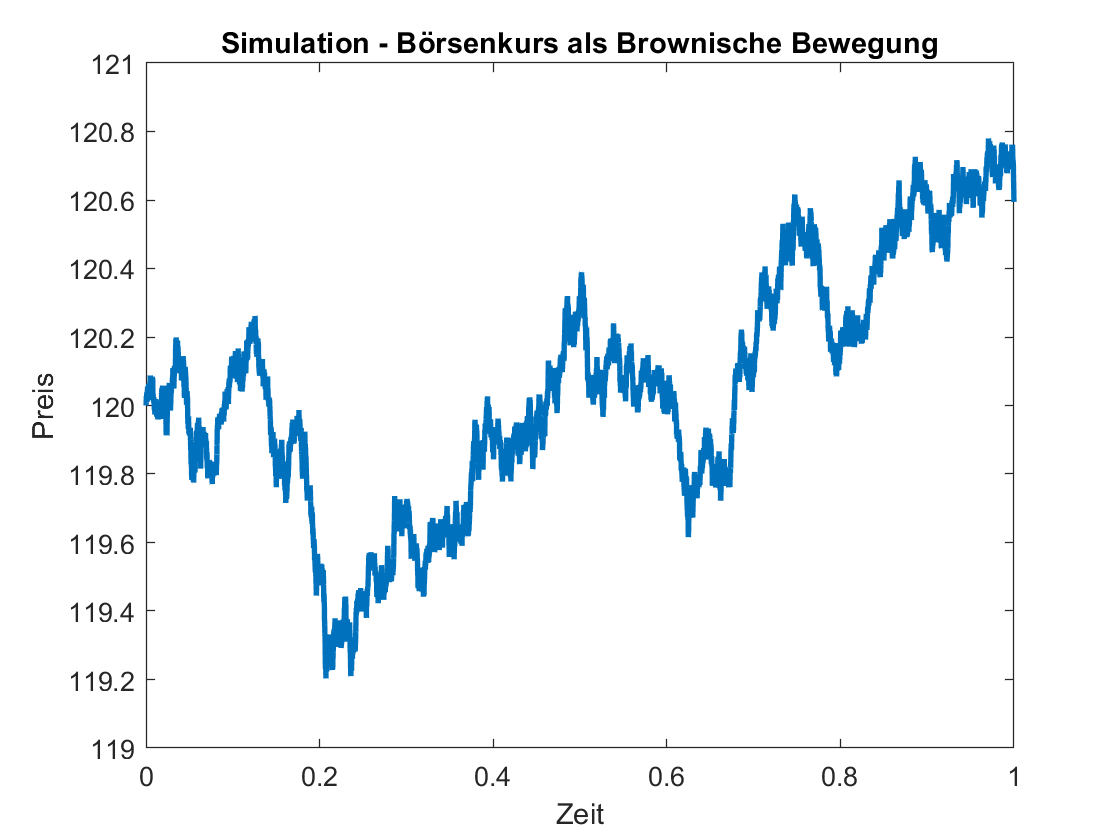
\includegraphics[width=\linewidth]{papers/brown/images/Aktienkurs-als-Brownische-Bewegung_3.png}
		\caption{Aktienkurs als 1D brownsche Bewegung}
		\label{1Dbrownian}
	\end{minipage}
	\hspace{0.05\linewidth}
	\begin{minipage}{0.45\textwidth}
		\centering
		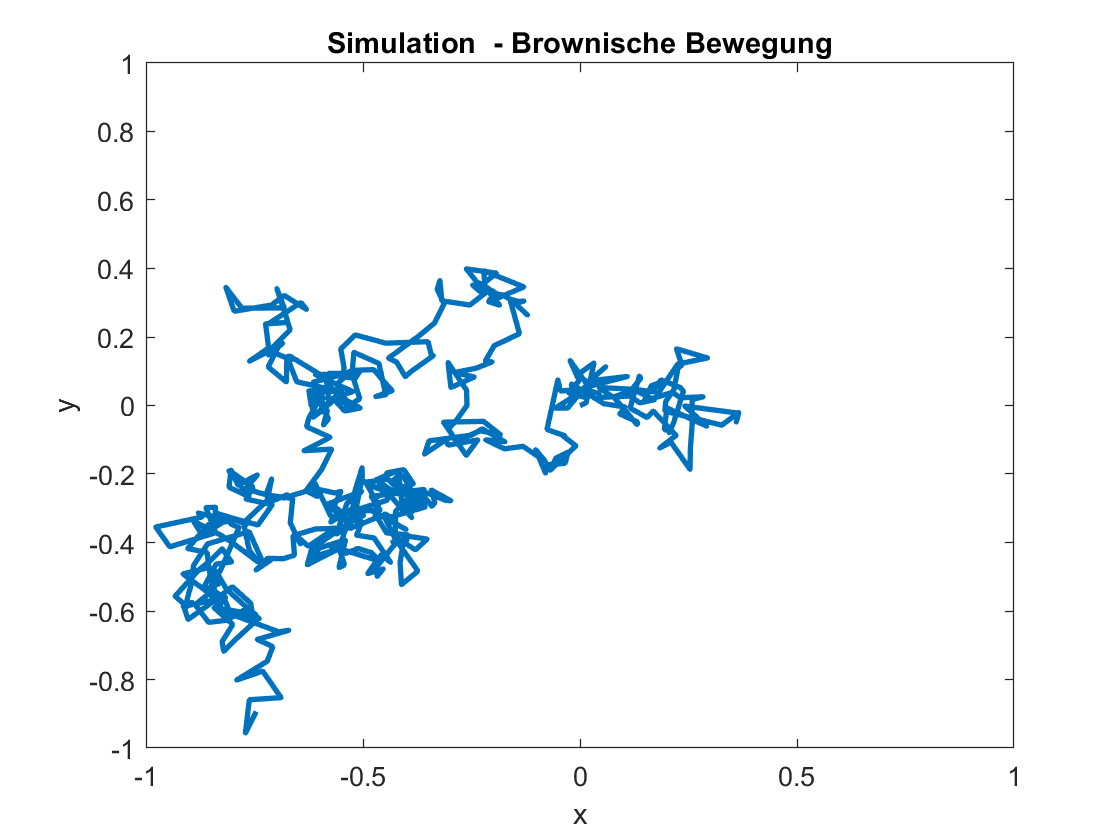
\includegraphics[width=\linewidth]{papers/brown/images/Brownische-Bewegung-Simuliert_3.png}
		\caption{Brownschen Bewegung simultiert in 2D}
		\label{2Dbrownian}
	\end{minipage}
\end{figure}

\subsection{ITO\label{brown:ito}}
\rhead{Ito} %Kurz-Titel der Section

Itō Kiyoshi war ein japanischer Mathematiker, der seine Kariere der Stochastik widmete und heute als Begründer der stochastischen Analysis erachtet werden kann. So legte er auch einen Grossteil des Fundaments auf dem der Umgang mit stochastische Differenzialgleichungen beruht. 

Nach ihm ist auch die \textit{Itō'sche Form} einer SDGL benannt, bei welcher die Gleichung mit dem Nenner des Differenzialquotienten multipliziert wird. Diese Form ist Ausgangslage viele seiner Konzepte, bietet jedoch auch den Vorteil, dass keine Differenzierbarkeit suggeriert wird.

Ein wichtiges Werkzeug, um mit stochastischen DIfferenzialgleichungen umzugenhen ist das Äquivalent zur Kettenregel, dem sogenannten \textit{Lemma von Ito}. %Dieses wird auch im Abschnitt XXXX für das Black-Scholes-Merton Modell verwendet. Auch nach ihm benannt ist die "ito-Form", in welcher die Gleichungen notiert sind XXX.%


Hier ein Beispiel einer stochastischen Differentialgleichung (SDGL) für einen Prozess X(t) in \textit{Ito-Form}:
\begin{equation}
	dX = a(X,t) dt + b(X,t) dW
\end{equation}


Angenommen, wir haben eine Funktion f(X,t), wobei X die Lösung der obigen SDGL ist, dann kann die Änderung von $ f $ in Bezug auf $ X $ und $ t $ wie folgt geschrieben werden:

Die Funktion f(X,t) und das \textit{Ito-Lemma}:
\begin{equation}
	df = \frac{\partial f}{\partial t} dt + \frac{\partial f}{\partial X} dX + \frac{1}{2} \frac{\partial^2 f}{\partial X^2} (dX)^2	
\end{equation}

Dieses Lemma erlaubt es uns, Differentialgleichungen für Funktionen von stochastischen Prozessen abzuleiten, was bei der Lösung von SDGs hilfreich ist.


Das Einsetzen der SDG in das Ito-Lemma ergibt:
\begin{equation}
	df = \frac{\partial f}{\partial t} dt + \frac{\partial f}{\partial X} (a dt + b dW) + \frac{1}{2} \frac{\partial^2 f}{\partial X^2} (b^2 dt)
\end{equation}

Die Funktion $ a(X,t) $ ist der \textit{Drift-Term}, der den deterministischen Teil der Bewegung darstellt, während $ b(X,t) $ der sogenannte \textit{Diffusions-Term} ist, welcher den stochastischen Teil der Bewegung darstellt.


%Gemäss Itō ist das Integral einer gewöhnlichen SDGL folgendermassen definiert:
%Weglassen?